\documentclass[11pt]{beamer}
\usepackage[utf8]{inputenc}
\usepackage[T1]{fontenc}
\usepackage[french]{babel}
\usepackage{amsmath}
\usepackage{amsfonts}
\usepackage{amssymb}
\usepackage{graphicx}
%\usepackage{siunitx}
\usepackage{multimedia}
\usepackage{subfig}
\usepackage[squaren,Gray]{SIunits}

\usetheme{Pittsburgh}

\usefonttheme{serif}

\begin{document}
	\author{Laura Guislain \and Nicolas Lecoeur \and André Kalouguine}
	\title{Étude du mouvement de colloïdes et de bactéries.}
	\titlegraphic{\includegraphics[height=1cm]{logo_ens}}
	\institute{E.N.S. de Lyon}
	%\date{}
	\subject{Caractérisation du mouvement bactérien et comparaison au mouvement brownien.}
	%\setbeamercovered{transparent}
	\setbeamertemplate{footline}{\hspace{0.5em}\insertframenumber}
	\setbeamertemplate{navigation symbols}{}
	\setbeamertemplate{caption}[numbered]
	\addtobeamertemplate{footline}{\vspace{-0.5em}}{\vspace{0.5em}}
\begin{frame}[plain]
	\maketitle
\end{frame}
\addtocounter{framenumber}{-1}

%\frame{\tableofcontents}

\section{Méthode expérimentale}

\begin{frame}{Mouvement brownien}
\renewcommand{\figurename}{Film}
\begin{figure}
	\centering
    \movie[height=6cm,poster]{Le film ne s'affichera pas dans ce lecteur pdf}{film_mvt_10s_400_images.avi}
    \caption{Mise en avant du mouvement brownien pour des colloïdes de 1$\micro \meter$ de diamètre.}
    \label{fig:movie_col}
\end{figure}
\end{frame}

\begin{frame}{Mouvement de bactéries}
\begin{figure}
\renewcommand{\figurename}{Film}
	\centering
	\movie[height=6cm,poster]{Le film ne s'affichera pas dans ce lecteur pdf}{film1.mp4}
	\caption{Mise en avant du mouvement de bactéries.}
	\label{fig:movie_bac}
\end{figure}
\end{frame}

\begin{frame}{Cellules d'observation}
\begin{columns}
	\column{0.5\linewidth}
	\begin{figure}
		\centering
		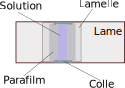
\includegraphics[width=\linewidth]{Cellule1}
		\caption{Premier modèle de cellule}
		\label{fig:cellule1}
	\end{figure}
	
	\column{0.5\linewidth}
	\begin{figure}
	\centering
	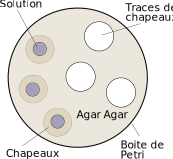
\includegraphics[width=\linewidth]{Cellule2}
	\caption{Second modèle de cellule}
	\label{fig:cellule2}
	\end{figure}
\end{columns}
\end{frame}

\begin{frame}{Microscope et caméra}
	\begin{figure}
    	\centering
    	\includegraphics[width=0.8\linewidth]{microscope.png}
    	\caption{Microscope utilisé}
    	\label{fig:microscope}
	\end{figure}

\end{frame}

\section{Étude préliminaire du mouvement en milieu simple}


\subsection{Mouvement brownien de colloïdes petits}

\begin{frame}{Mouvement brownien}
\framesubtitle{Observation du mouvement}
	\begin{figure}
		\centering
		\includegraphics[width=0.9\linewidth]{Trajectory_brownian}
		\caption{Trajectoire d'un colloïde sur 4000 points ($f=$ 400 \hertz)}
		\label{fig:trajectory_b}
	\end{figure}
\end{frame}

\begin{frame}{Mouvement brownien}
\framesubtitle{}

$$ \Delta x (t, \tau) = x (t + \tau ) - x(t)$$
\begin{figure}
	\centering
	\includegraphics[width=0.7\linewidth]{delta_x_t_tau_}
	\caption{Courbes représentant le déplacement $\Delta x $ pour différents $\tau$.}
	\label{fig:deltaxttau}
\end{figure}
\end{frame}


\begin{frame}{Mouvement brownien}
\framesubtitle{Limite de $\tau$}
\begin{figure}
	\centering
	\includegraphics[width=0.8\linewidth]{collo_histogramme_diff_tau}
	\caption{Histogrammes représentant la répartition des $\Delta x $ pour différents $\tau$.}
	\label{fig:collo_histogramme_diff_tau}
\end{figure}
\end{frame}


\begin{frame}{Mouvement brownien}
\framesubtitle{Corrélation}
	\begin{figure}
		\centering
		\includegraphics[width=0.9\linewidth]{Correlation_brownian}
		\caption{Fonction d'autocorrélation}
		\label{fig:correl_b}
	\end{figure}
\end{frame}



\begin{frame}{Mouvement brownien}
\framesubtitle{Ecart-type}

Mettre sgma2 en fonction de tau2 en entier ! 

\end{frame}


\begin{frame}{Mouvement brownien}
\framesubtitle{Coefficient de diffusion - Méthodes}
\begin{columns}
    \column{.5\linewidth}
	\begin{figure}
\includegraphics[width=1\linewidth]{graphe_y.png}
\caption{$\sigma_y^2 = f(\tau)$. }
\end{figure}
    
    \column{.5\linewidth}
        \begin{figure}
        \includegraphics[width=1\linewidth]{graphe_y_log.png}
        \caption{$\ln(\sigma_y^2) = f(\ln\tau)$.}
        \end{figure}
\end{columns}
\vspace{0.5cm}
\centering Loi théorique : $\sigma_y^2 = 2D\tau$\end{frame}

\begin{frame}{Mouvement brownien}
\framesubtitle{Coefficient de diffusion - Résultats}
\begin{itemize}
\item Relation de Stokes-Einstein : 
\begin{equation*}
D = \frac{kT}{6\pi \eta a} = \unit{0.429}{\micro\meter^2 \reciprocal \second}
\end{equation*}
avec $a = \unit{0.5}{\mu\meter}$ le rayon des colloïdes. 
\item Par régressions linéaires en échelle réelle : 
\begin{equation*}
D = \unit{0.42 \pm 0.04}{\micro\meter^2 \reciprocal \second} \text{ à 95\%}
\end{equation*}
\item Par régressions linéaires en échelle logarithmique : 
\begin{equation*}
D = \unit{0.42 \pm 0.05}{\micro\meter^2 \reciprocal \second} \text{ à 95\%}
\end{equation*} 
\end{itemize}
\end{frame}


\begin{frame}{Mouvement brownien}
\framesubtitle{Symétrie de la distribution}
\begin{columns}
    \column{.5\linewidth}
    \begin{figure}
    \centering
    \includegraphics[width=0.75\linewidth]{exemples_skewness_2.png}
    \caption{Skewness et asymétrie.}
    \label{fig:skewness}
    \end{figure}
    
	
	\column{.5\linewidth}
	\begin{figure}
    	\centering
    	\includegraphics[width=0.9\linewidth]{m_3.png}
    	\caption{Moment d'ordre 3}
    	\label{fig:moment3}
	\end{figure}
\end{columns}
\end{frame}

\begin{frame}{Mouvement brownien}
\framesubtitle{Ecart de la distribution à la gaussienne}
\begin{columns}
    \column{.5\linewidth}
	\begin{figure}
	\centering
	\includegraphics[width=0.9\linewidth]{exemples_kurtosis_3.png}
	\caption{Kurtosis et aplatissement.}
	\label{fig:kurtosis}
	\end{figure}
	
	\column{.5\linewidth}
	\begin{figure}
    	\centering
    	\includegraphics[width=0.9\linewidth]{m_4.png}
    	\caption{Moment d'ordre 4}
    	\label{fig:moment4}
	\end{figure}
\end{columns}
\end{frame}

\begin{frame}{Mouvement brownien}
\framesubtitle{Conclusion}
- permet de valider le tracking et la façon dont on étudie la trajectoire
-applications : déduit $\eta$ pour un solvant --> viscosimètre
            carcatérise a le rayon : meilleure résolution qu'avec un microscope
\end{frame}


\subsection{Mouvement des bactéries vivantes}


\begin{frame}{Mouvement bactérien}
\begin{center}
    \begin{tabular}{cc}
    \setlength\tabcolsep{-2cm}
    \includegraphics[scale=0.3]{Trajectory_bac_1} & \includegraphics[scale=0.3]{Trajectory_bac_16} \\
    \includegraphics[scale=0.3]{Trajectory_bac_4} & \includegraphics[scale=0.3]{Trajectory_bac_5} \\
    Trajectoires droites & Trajectoires courbees
    \end{tabular}
    \end{center}
\end{frame}

\begin{frame}{Mouvement brownien}
\framesubtitle{Lissage}
\begin{figure}

%\includegraphics[scale = 0.14]{trajectoire_bacterie1_video_gras.png}
%\includegraphics[scale = 0.14]{trajectoire_bacterie1_video_lisse_gras.png}
\includegraphics[width=0.9\textwidth]{Trajectory_lisse}
\caption{Lissage de la trajectoire.}
\end{figure}
\end{frame}

\begin{frame}{Mouvement bactérien}
\framesubtitle{Trajectoire droite}

\begin{columns}
\column{.5\linewidth}
\begin{figure}
\centering
\includegraphics[width=1\linewidth]{traj_lissee.png}
\caption{Trajectoire lissée.}
\end{figure}

\column{.6\linewidth}
\begin{figure}
\centering
\includegraphics[width=0.82\linewidth]{vitesse_v_1.png}
\caption{Vitesse en fonction du temps.}
\label{fig:my_label}
\end{figure}
\end{columns}
\begin{equation*}
v = \unit{13,9}{\micro\meter\reciprocal\second} \text{ d'écart-type } \sigma = \unit{3,1}{\micro \meter\reciprocal\second}
\end{equation*}


\end{frame}


\begin{frame}{Mouvement bactérien}
\framesubtitle{Trajectoire droite}

\begin{figure}
\includegraphics[width=0.6\linewidth]{vitesse_v_log_pente_non_forcee1.png}
\caption{$\sigma ^2$ en fonction de $\tau ^2$.}
\end{figure}
il faut aussi mettre le graph avec la pente forcée à 1, et de la on en déduit le vrai v!
Loi théorique : $\sigma ^2 = v^2\tau ^2$ conduit à $v = \unit{13,032 \pm 0,005}{\micro\meter\reciprocal\second}$
\end{frame}

\begin{frame}{Mouvement bactérien}
\framesubtitle{Trajectoire circulaire}
\begin{columns}
\column{.5\linewidth}
\begin{figure}
\centering
\includegraphics[width=1\linewidth]{traj_lissee_1.png}
\caption{Trajectoire lissée.}
\end{figure}

\column{.5\linewidth}
\begin{figure}
\includegraphics[width=1\linewidth]{dx2_t2_log_5.png}
\caption{$ln(\sigma ^2)$ en fonction de $ln(\tau ^2)$.}
\end{figure}

\end{columns}
\end{frame}


\begin{frame}{Mouvement bactérien}
\framesubtitle{Trajectoire circulaire - Rayon de courbure}
\begin{columns}
\column{0.5\textwidth}
\begin{figure}
\includegraphics[width=1\linewidth]{rayon_de_courbure.jpg}
\caption{Rayon de courbure - Définition.}
\end{figure}
\column{0.5\textwidth}
\begin{figure}
\includegraphics[width=1\linewidth]{rayon.png}
\caption{Rayon de courbure de la trajectoire lissée.}
\end{figure}
\end{columns}
\end{frame}



\begin{frame}{Mouvement bactérien}
\framesubtitle{Longueur de persistance - Définition}
\begin{figure}
\includegraphics[width=0.9\linewidth]{longueur_persistance.jpg}
\caption{Fonction d'autocorrélation : $g(s) = \langle \overrightarrow{t}(s)\cdot\overrightarrow{t}(0)\rangle$.}
\end{figure}
Longueur de persistance : $L_p$ telle que si $s\gtrsim L_p$ alors $\lvert g(s)\rvert \ll 1$.
\end{frame}

\begin{frame}{Mouvement bactérien}
\framesubtitle{Longueur de persistance - Détermination}
\begin{figure}
\includegraphics[width=0.9\linewidth]{Correlation_bactery.png}
\caption{Fonction de correlation sur la trajectoire.}
\end{figure}
\end{frame}





\section{Étude du mouvement autour de colloïdes ou qqch d'autre}




\appendix
\begin{frame}
ANNEXE
\end{frame}
\begin{frame}{Hermiticité de nos cellules}
Faire un graphique avec + de cellules.
\begin{figure}
	\centering
	\includegraphics[width=0.8\linewidth]{FuitesNico_1}
	\caption{Mouvement général des colloïdes dans une cellule. Si le module est proche de 1, alors $\mu$ comparabale devant $\sigma$}
	\label{fig:fuitesnico1}
\end{figure}
\end{frame}

\end{document}